%%%
%%% Carsten Gips, FH-Bielefeld
%%% 05.09.2015
%%%
%%%

%------------------------------------- Klasse ---------------------
%%% Beamer: Slides
\documentclass[svgnames,smaller,ngerman]{beamer}
%------------------------------------- Klasse ---------------------


%------------------------------------- Theme ---------------------
\usetheme{default}
\usecolortheme{rose}

% keine Navigationsleiste
\setbeamertemplate{navigation symbols}{}

% schmalere Ränder
\setbeamersize{text margin left=4mm}
\setbeamersize{text margin right=4mm}

% extra Folie für Ueberschrift
\AtBeginSection{
  \let\insertsectionnumber\relax
  \let\sectionname\relax
  \frame{\sectionpage}
}

% colors: white text on 90% black background
\setbeamercolor{normal text}{fg=black!70,bg=white}

% light blue as a highlight color
\setbeamercolor*{structure}{fg=midnightblue!90}
\setbeamercolor*{palette primary}{use=structure,fg=structure.fg}
\setbeamercolor*{palette secondary}{use=structure,fg=structure.fg!95!black}
\setbeamercolor*{palette tertiary}{use=structure,fg=structure.fg!90!black}
\setbeamercolor*{palette quaternary}{use=structure,fg=structure.fg!95!black,bg=black!80}

\setbeamercolor*{framesubtitle}{fg=white}
%------------------------------------- Theme ---------------------


%------------------------------------- Sprache, Encoding, Font ----------------
\usepackage[english,ngerman]{babel}
\usepackage[utf8]{inputenc}
\usepackage[T1]{fontenc}
\usepackage[babel]{csquotes}

\usepackage{mathptmx}
\usepackage[scaled=.92]{helvet}
\usepackage{courier}
%------------------------------------- Sprache, Encoding, Font ----------------


%------------------------------------- Pakete ---------------------
\usepackage{amsmath,amsfonts,amssymb}

\usepackage{graphicx}
\usepackage{pgf}

\usepackage{hyperref}
\usepackage{xspace}

\usepackage{listings}
%------------------------------------- Pakete ---------------------


%------------------------------------- Befehle ---------------------
\newcommand{\blueArrow}{{\color{midnightblue}$\pmb{\Rightarrow}$}\xspace}

\newcommand{\columnsbegin}{\begin{columns}}
\newcommand{\columnsend}{\end{columns}}
\newcommand{\minipagebegin}{\begin{minipage}}
\newcommand{\minipageend}{\end{minipage}}
\newcommand{\centerbegin}{\begin{center}}
\newcommand{\centerend}{\end{center}}

\newsavebox{\mynotebox}
\newcommand{\usemynotebox}{\usebox{\mynotebox}}
\newenvironment{mynotes}[1][\textwidth]{\begin{lrbox}{\mynotebox}\begin{minipage}{#1}}{\end{minipage}\end{lrbox}\usemynotebox}
\newcommand{\notesbegin}{\begin{mynotes}}
\newcommand{\notesend}{\end{mynotes}}

\newsavebox{\mycolorbox}
\newenvironment{mycbox}{\begin{lrbox}{\mycolorbox}}{\end{lrbox}\begin{center}\fcolorbox{blue}{listinggray}{\usebox{\mycolorbox}}\end{center}}
\newcommand{\cboxbegin}{\begin{mycbox}}
\newcommand{\cboxend}{\end{mycbox}}
%------------------------------------- Befehle ---------------------


%------------------------------------- Befehle ---------------------
\newcommand{\bsp}[1]{\vfill\hfill\beamerbutton{#1}}
\newcommand{\Alert}[1]{\alert{\textbf{#1}}\xspace}
\renewcommand{\usemynotebox}{}  % keine Notes
%------------------------------------- Befehle ---------------------


%------------------------------------- Farben ---------------------
\usepackage{xcolor}
\definecolor{dkgreen}{rgb}{0,0.6,0}
\definecolor{dkred}{rgb}{0.6,0,0}
\definecolor{dkblue}{rgb}{0,0,0.6}
\definecolor{gray}{rgb}{0.7,0.7,0.7}
\definecolor{listinggray}{gray}{0.92}
\definecolor{midnightblue}{rgb}{0.2,0.2,0.7}
%------------------------------------- Farben ---------------------


%------------------------------------- Listings ---------------------
%% Einstellungen fuer alle Listings (Package-Import in Template)
\lstset{basicstyle=\small\ttfamily\mdseries, xleftmargin=\bigskipamount, keywordstyle=\bfseries\color{dkblue}, identifierstyle=\ttfamily, commentstyle=\bfseries\color{gray}\textsl, stringstyle=\color{magenta}\upshape, emphstyle=\color{red}, emphstyle={[2]\color{blue}}, texcl=false, showspaces=false, showstringspaces=false, numbers=left, numberstyle=\footnotesize, breaklines=true, tabsize=4, backgroundcolor=\color{listinggray}, frame=shadowbox}

%% Latex-Keywords
%\lstset{morekeywords={subtitle, institute, logo, titlegraphic, subject, keywords, author, document, subfigure, chapter, section, subsection,subsubsection, paragraph, tiny, small, itemize, description, enumerate, lsubset, boolean, setboolean, ifthen, lengthtest, equal, IfFileExists, InputIfFileExists, AtBeginDocument, AtEndDocument, DefinesOption, ProcessOptions, ExecuteOption, ProvidesPackage, RequirePackage, align, center, minipage, includegraphics, maketitle, tableofcontents, equation, cases}}

%% Scala-Keywords: Scala wird von Listings nicht unterstützt?!
\lstset{morekeywords={class, object, trait, extends, override, new, def, val, var, for, yield, if, else, require, with, match, case}}

%% Ruby/IO-Keywords
%\lstset{morekeywords={print,Object,clone,slotNames,type,method,proto,getSlot,block,super,resend,OperatorTable,addOperator,call,sender,target,message,doMessage,forward}}

%% Java-Keywords
%\lstset{morekeywords={project,target,echo,property,javac,delete,copy,fileset,dirset,include,exclude,classpath,pathelement,junit,test,batchtest,formatter,junitreport,report}}


%% Code-Befehl (Code im Text: lieber grün und fett als texttt und klein)
%% => DEPRECATED!
\newcommand{\code}[1]{\textcolor{dkgreen}{\texttt{\textbf{#1}}}\xspace}
%------------------------------------- Listings ---------------------


%------------------------------------- Infos ---------------------
\title{VL06: Haskell (Funktionen höherer Ordnung, Currying)}
\subtitle{IFM 5.3 Spezielle Methoden der Programmierung}
\author{Carsten Gips, FH Bielefeld}
\date{18.05.2015}
%------------------------------------- Infos ---------------------


%------------------------------------- Dokument ---------------------
\begin{document}

% Titelseite
\frame{
    \titlepage
}



% Wiederholung
\section{Wiederholung}

\begin{frame}[fragile]{Wiederholung}
    \begin{itemize}
        \item Wie können Sie die ersten $n$ Elemente einer Liste auswählen?
        \item Wie können Sie die ersten $n$ Elemente einer Liste entfernen?
        \item Was sind \enquote{List Comprehensions}?
        \item Was ist der Unterschied zwischen den beiden folgenden Aufrufen?
        \begin{small}
        \begin{lstlisting}[language=Haskell]
zip [1 .. 5] ["one", "two", "three"]
[(x, y) | x <- [1 .. 5], y <- ["one", "two", "three"]]
        \end{lstlisting}
        \end{small}
        \item Was bedeutet \enquote{Pattern Matching} im Zusammenhang mit der
        Funktionsdefinition?
    \end{itemize}
\end{frame}



% Motivation
\section{Motivation}

\begin{frame}[fragile]{Themen für heute}
    \begin{center}
    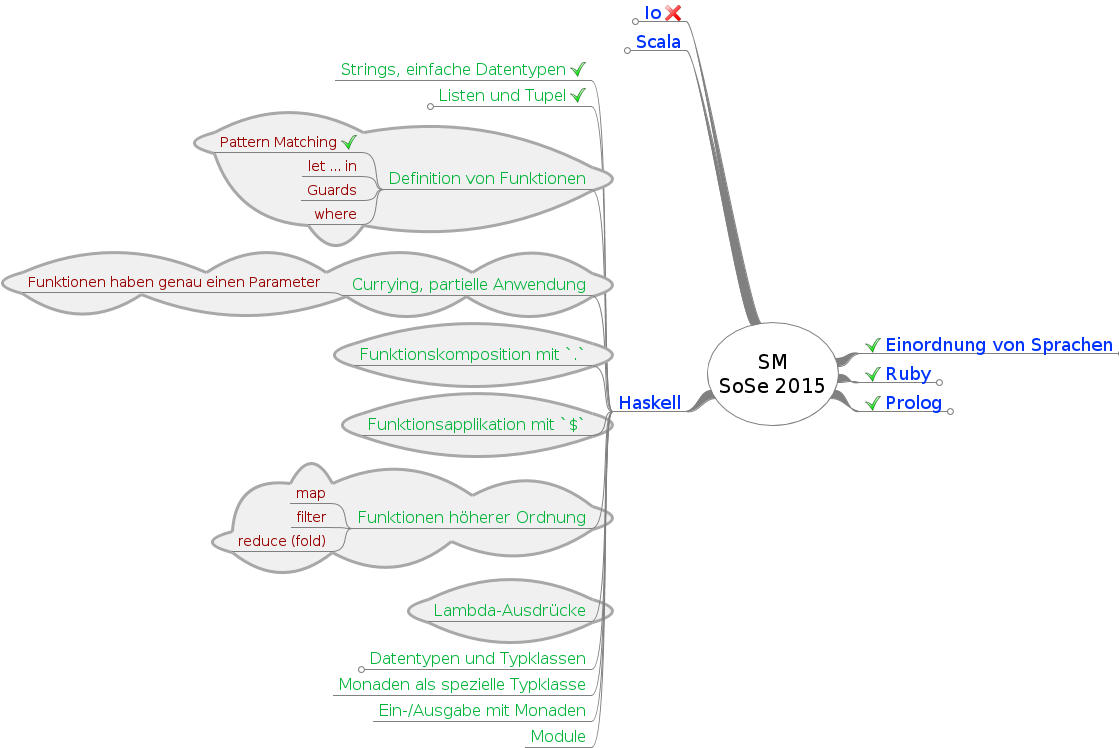
\includegraphics[width=90mm]{figs/themen-sm.png}
    \end{center}

    \begin{itemize}
        \item Funktionen mit Guards und \verb/where/ definieren
        \item Currying und partiell angewendete Funktionen
        \item Funktionen höherer Ordnung: Faltungen, Map, Filter, Lambda-Ausdrücke
    \end{itemize}

    \bsp{Mindmap}
\end{frame}



% Kapitel: Weitere Formen der Verarbeitung von Listen
\section{Weitere Formen der Verarbeitung von Listen}

\begin{frame}[fragile]{List Comprehensions (Listenverarbeitung)}
    \begin{columns}
    \column{0.48\textwidth}

    $$
    S = \left\{ 2*x \;|\;\; x \in N, x \le 10 \right\}
    $$

    \column{0.48\textwidth}
    \pause
    \bigskip
    \medskip

    \begin{small}
    \begin{lstlisting}[language=Haskell]
[x*2 | x <- [1..10]]
    \end{lstlisting}
    \end{small}

    \end{columns}

    \pause
    \bigskip
    \bigskip
    \bigskip
    \begin{lstlisting}[language=Haskell]
Prelude> [x*2 | x <- [1..10], x*2>5]

Prelude> let xs = ["A", "B", "C"]
Prelude> [a ++ "-" ++ b | a <- xs, b <- xs]
Prelude> [a ++ "-" ++ b | a <- xs, b <- xs, a < b]

Prelude> [(a,b) | a <- [1..3], b <- [1..a]]
    \end{lstlisting}

    \mode<article>
    \begin{itemize}
        \item List Comprehensions ergeben eine Liste
        \item Linke Seite: Ausdruck, der zum Bilden der Listenelemente genutzt
              wird
        \item Rechte Seite:
        \begin{itemize}
            \item Generatoren: \verb/a <- xs/ bedeutet \enquote{Nimm der Reihe
                  nach alle Elemente aus \texttt{xs} und binde sie an
                  \texttt{a}}
            \item Filter: Prädikate, die erfüllt sein müssen, damit das aktuell
                  betrachtete Element aus dem Generator in die Ergebnisliste
                  übernommen wird
        \end{itemize}
        \item Pattern Matching funktioniert auch in List Comprehensions:
              \verb/[a+b | (a,b) <- xs]/
    \end{itemize}
    \mode<all>

    \bsp{ghci}
\end{frame}


\begin{frame}[fragile]{Beispiel zipWith-Funktion}
    \begin{itemize}
        \item Eingabe: Funktion $f$, zwei Listen
        \item Rückgabe: Liste
        \item Arbeitsweise: Fügt die Listen zusammen, indem für die
              korrespondierenden Elemente jeweils die Funktion  $f$ aufgerufen
              wird
    \end{itemize}

    \smallskip

    \Alert{Signatur?}
    \pause
    \begin{small}
    \begin{lstlisting}[language=Haskell]
zipWith :: (a -> b -> c) -> [a] -> [b] -> [c]
    \end{lstlisting}
    \end{small}

    \Alert{Definition?}
    \pause
    \begin{small}
    \begin{lstlisting}[language=Haskell]
zipWith _ [] _ = []
zipWith _ _ [] = []
zipWith f (x:xs) (y:ys) = f x y : zipWith f xs ys
    \end{lstlisting}
    \end{small}

    \mode<article>
    \Alert{Anwendung:}
    \begin{small}
    \begin{lstlisting}[language=Haskell]
Prelude> zipWith (+) [4,2,5,6] [2,6,2,3]
Prelude> zipWith max [6,3,2,1] [7,3,1,5]
    \end{lstlisting}
    \end{small}
    \mode<all>

    \bsp{ghci}
\end{frame}


\begin{frame}{Berechnung der Aktivierung von Neuron \(a_j\)}
    Aktivierung von Neuron \(a_j\):

    \[a_j = \left\{
    \begin{array}{lll}
        1 & \text{ falls } & w_{0,j} + a_1 w_{1,j} + a_2 w_{2,j} + ... + a_n w_{n,j} \ge 0\\
        0 & \text{ falls } & w_{0,j} + a_1 w_{1,j} + a_2 w_{2,j} + ... + a_n w_{n,j} < 0
    \end{array}
    \right.\]
\end{frame}


% Zusammenfassung
\section{Zusammenfassung}

\begin{frame}[fragile]{Was haben Sie heute gehört?}
    \begin{itemize}
        \item Funktionsdefinition mit Guards, mit Where-Bindings und Let-in
        \item Funktionen haben in Haskell genau \textbf{einen} Parameter
        \item \textbf{Currying}: Partielle Anwendung einer Funktion auf einen
              Parameter liefert Funktion mit restlichen Parametern
        \item Funktionskomposition mit \verb/./
        \item Funktionen höherer Ordnung: Funktionen als Parameter oder
              Rückgabe\\
              \blueArrow Beispiele: \verb/map/, \verb/filter/, \verb/foldl/
              (\enquote{reduce})
        \item Anonyme Funktionen mit Lambda-Ausdrücken
    \end{itemize}

    \vfill

    \textbf{Nächste Woche}: Haskell (Typen und Typklassen)
\end{frame}


\begin{frame}{Literatur zum Weiterlesen}
    \begin{itemize}
        \item Miran Lipovaca: \enquote{Learn You a Haskell for Great Good!},
              \href{http://learnyouahaskell.com}{learnyouahaskell.com}
        \item O’Sullivan, Stewart, Goerzen: \enquote{Real World Haskell},
              \href{http://book.realworldhaskell.org}{book.realworldhaskell.org}
        \item Bruce A. Tate: \enquote{Seven Languages in Seven Weeks},
              Pragmatic Bookshelf Inc., 2010
              \begin{itemize}
                  \item Haskell: Kapitel 8
              \end{itemize}
        \item Block, Neumann: \enquote{Haskell Intensivkurs}, Springer, 2011
    \end{itemize}
\end{frame}


\begin{frame}[fragile]{Lernziele -- Nach dieser Vorlesung sollten Sie \ldots}
    \begin{block}{Verstehen (K2)}
        \begin{itemize}
            \item Funktionen haben in Haskell einen Parameter
            \item Prinzip des Currying (schrittweise partielle Applikation)
            \item Signatur von Funktionen höherer Ordnung
            \item Currying oft lesbarer als Lambda-Ausdrücke
        \end{itemize}
    \end{block}

    \smallskip

    \begin{block}{Anwenden (K3)}
        \begin{itemize}
            \item Funktionsdefinition mit Guards und Pattern Matching
            \item Nutzung von Where-Bindings und Let-in
            \item Komposition von Funktionen mit \verb/./
            \item Umgang mit \verb/map/, \verb/filter/, \verb/foldl/,
                  \verb/zip/, \ldots
            \item Nutzung von Lambda-Ausdrücken
        \end{itemize}
    \end{block}
\end{frame}


\begin{frame}{Diese Fragen sollten Sie beantworten können \ldots}
    \begin{itemize}
        \item Worin besteht der Unterschied zwischen Guards und Pattern
              Matching?
        \item Worin besteht der Unterschied zwischen Where-Bindings und
              Let-in-Ausdrücken?
        \item Erklären Sie Currying an einem Beispiel. Worin liegt die
              praktische Bedeutung von partieller Applikation?
        \item Was sind Lambda-Ausdrücke?
    \end{itemize}
\end{frame}


\begin{frame}[fragile]{Diese Fragen sollten Sie beantworten können \ldots}
    \begin{itemize}
        \item Erklären Sie \verb/foldl/ an einem Beispiel.
        \item Was bedeuten die folgenden Code-Schnipsel?
            \begin{small}
            \begin{lstlisting}[language=Haskell]
map (+ 1) [1, 2, 3]
filter odd [1, 2, 3, 4, 5]
foldl1 (+) 0 [1 .. 3]
            \end{lstlisting}
            \end{small}
    \end{itemize}
\end{frame}


\begin{frame}[fragile]{Diese Fragen sollten Sie beantworten können \ldots}
    \begin{itemize}
        \item Schreiben Sie im folgenden Code-Schnipsel \verb/fibNth/ mit Hilfe
              von Funktionskomposition um:
            \begin{small}
            \begin{lstlisting}[language=Haskell]
lazyFib x y = x:(lazyFib y (x + y))
fib = lazyFib 1 1
fibNth x = head (drop (x - 1) (take (x) fib))
            \end{lstlisting}
            \end{small}
        \item Definieren Sie eine Funktion \verb/fib5th/ durch partielle
              Applikation.
    \end{itemize}
\end{frame}



\end{document}
%------------------------------------- Dokument ---------------------
